\pagestyle{fancy}
\fancyhead[LE,LO]{OCR A Level - Computer Science NEA}
\fancyhead[RE,RO]{Jonathan Kasongo}

\chapter{Analysis of the problem}

\section{Problem Identification}
% Describe and justify features of the problem that make it 
% solvable by computational methods, explaining why it's 
% amenable to a computational approach.
\subsection*{Description of the problem}
The current process of studying chess using an engine can 
definitely be improved. Commonly used websites like
\url{chess.com} have other good study features hidden behind
a paywall. \footnote{\url{https://www.chess.com/membership}}
Moreover there is no easy way to take notes on a certain 
position on this website making note taking whilst you study 
chess more undesirable to beginner level players.
It is no secret that a chess engine is an invaluable tool 
when studying chess. That being said the current de facto
standard of chess engine programs "Stockfish" lacks ease 
of use for users that aren't familiar with compiling \texttt{C++} 
programs. This can also seem intimidating to some users who
are used to applications with graphical user interfaces 
seeing as stockfish is entirely terminal 
based. \cite{stockfish} In order to connect to a user interface
one must install another memory-hungry application, \textit{Surely}
there should be an application that provides a graphical user
interface and a chess-engine in one?

\subsection*{Desired Solution}
I aim to write a chess engine capable of beating the 
average chess player at my school 9 times out of 10 for 
one of my classmates John Arco, to help him to study
chess strategies and tactical ideas effectively and to
be able to defeat the best chess players in our school. \\


The engine should also be familiar and easy to use. This
means that it should not require any programming experience
to install and use it, and it should also have a graphical 
user interface that is intuitive and easy to use. The interface
should allow for the user to drag and drop pieces onto the square 
they choose.\\


The engine should perform at a rating of >1000 ELO. It 
should also provide an analysis board where the evaluation
of a position is given so the user can learn to find the moves
that are optimal for a give position position. The application should
also provide a way to simply take notes on a position on the
board, to enrich the learning process.\\


The engine should also play chess accurately. That means
not making illegal moves and recognising when a player has
won, drawn or lost the game.

% Useful document on how to draw game trees with Tikz
% https://www.sfu.ca/~haiyunc/notes/Game_Trees_with_TikZ.pdf
%\begin{center}
%  \begin{tikzpicture}[level 1/.style={sibling distance=4.5cm},level 2/.style={sibling distance=2cm}]
%  \tikzstyle{w}=[circle,draw,inner sep=8]
%  \tikzstyle{b}=[circle,draw,inner sep=8,fill=darkgray]
  
%  \node[w,label=above:{Eval: +0.1}]{\large e4}
%    child{node[b,label=above:{Eval: +0.2},yshift=-0.7cm]{\large e5}
%      child{node[w,label=above:{Eval: +0.2},yshift=-0.7cm]{Nf3}}
%      child{node[w,label=above:{Eval: +0.1},yshift=-0.7cm]{Nc3}}
%    }
%    child{node[b,label=above:{Eval: 0.0},yshift=-0.7cm]{\large e6}
%      child{node[w,label=above:{Eval: +0.4},yshift=-0.7cm]{\large d4}}
%      child{node[w,label=above:{Eval: +0.2},yshift=-0.7cm]{Nf3}}
%    };
%\end{tikzpicture}
%\end{center}

\newpage
\section{Stakeholders}
% https://www.nytimes.com/2022/06/17/crosswords/chess/chess-is-booming.html
% Identify suitable stakeholders for the project and describe how will make
% use of the proposed solution and how it is appropiate to your needs.
One of the students at my school who plays chess regularly is 
John Arco. John Arco is a 17 year old male with a passion for chess.
John has a rating of roughly 1000 ELO but wishes 
to improve to a higher rating and beat all of his 
classmates. Not only does he want to test his strength against a 
chess engine he also recognises that using a chess engine can also be highly 
educational as we may learn new ideas or tactics from the engine that
we may have never considered previously. Even the world's rank 1 chess
player Magnus Carlsen has openly said that he has learnt new ideas
from chess engines. \cite{lex} This means the engine is to aid
the improvement of John Arco's chess ability by exposing him to 
new and unique tactics that he wouldn't have thought of otherwise. 
The construction of a strong chess engine program will be able to
facilitate John's growth effectively, providing both educational benefits and 
benefits to mental cognition skills also. \cite{cog} 

The following is a transcript of an interview I
conducted with my client John Arco on how he will make use of the
engine and how it is appropiate to his needs. This will 
help me to clearly understand the requirements and goals I
should keep in mind when programming.

\begin{tcolorbox}
\textbf{\texttt {Date: Tue April 9th 2024}}\\
\textbf{\texttt {Time: 10:30 UTC}}\\
\makebox[2cm]{\textbf{Jonathan:}} Hi John thanks for doing this interview. \par
\makebox[2cm]{\textbf{John:}} No worries \par 
\makebox[2cm]{\textbf{Jonathan:}} Why are you looking for a chess engine?\par
\makebox[2cm]{\textbf{John:}} I am looking to improve my
chess rating to around 2000 ELO, and a chess engine would
help me a lot.\par
\makebox[2cm]{\textbf{Jonathan:}} What features should this
engine have? \par
\makebox[2cm]{\textbf{John:}} The engine should definitely
play at a strength stronger than me, It should also include
an easy to use GUI and it can be written in any programming
language.\par
\makebox[2cm]{\textbf{Jonathan:}} How will you use the
engine? \par
\makebox[2cm]{\textbf{John:}} I will play games against the 
engine to practise and improve my rating, I will also use it
to review my games to help me see the mistakes in the moves 
that I played. \par
\makebox[2cm]{\textbf{Jonathan:}} How will the engine be 
appropiate to your needs? \par
\makebox[2cm]{\textbf{John:}} This engine will allow me to 
easily analyse my games from my laptop, and help me in 
achieving my goal of chess mastery in the process. \par
\makebox[2cm]{\textbf{Jonathan:}} Any other requirements for
the engine? \par
\makebox[2cm]{\textbf{John:}} It should be reliable and also 
be easy to install since I don't do computer science. \par
\end{tcolorbox}


\subsection*{Analysis of interview}
Based on the interview with my client I was able to get 
some clear features, that the finished program should
include. The request to have the engine play at a strength
of >1000 ELO, is no simple task so it will be split into
numerous sub-tasks that will aid me in designing the final 
program. \\

\textbf{\large Main requirement list:}
\begin{itemize}
  \item Be easy to use
  \item Include a clean user interface
  \item Play at a strength of >1000 ELO
  \item Be reliable and robust
  \item Have an easy installation process

  \begin{itemize}
    \item{Generate legal moves with a consistent and fast
          algorithm}
    \item Evaluate positions with heuristical optimisations
    \item{Search for moves with a suitably fast algorithm}
  \end{itemize}

\end{itemize}

More potential stakeholders and their goals are listed below.
\subsection*{Students from my school}
\begin{tblr}{Q[h]X}
  \altbf{Description:} & Avid chess players of varying skill 
  levels.\\
  \altbf{How will they use it?} & They may use it to test their
  strength against the engine, or to review their games.\\
\end{tblr}

\vspace{0.3cm}
\altbf{Why is it appropiate to their needs?}
\begin{itemize}
  \item They will be able to play games against the program
  \item{They will be able to analyse their games with an 
    analysis board}
\end{itemize}

\subsection*{Chess coaches}
\begin{tblr}{Q[h]X}
  \altbf{Description:} & Paid chess coaches and teachers that 
  have significant experience in the game of chess.\\
  \altbf{How will they use it?} & They may use it to challenge their
  students and to provide analysis of their students games.\\
\end{tblr}

\vspace{0.3cm}
\altbf{Why is it appropiate to their needs?}
\begin{itemize}
  \item{They will be able to take notes on positions to emphasise
    teaching points to the student}
  \item They will be able to observe as their student plays with the engine
\end{itemize}

I also conducted further interviews with other students
from my school. The students I chose all have some
background in chess at various skill levels. The following 
is some of the features they suggested. \newpage

\begin{center}
  \begin{tblr}{
    colspec = {XXXX},
    hline{1} = {0.1em, niceblue}, hline{2-Z} = {niceblue},
    row{1} = {lightgray},
  }
  Feature & Implementation & {How will the user interact
  with\\ the feature?} & {How does this meet the\\
  stakeholders needs?}\\
  %a & b & c & d \\
  Allow user to change the strength of the engine & {During 
  move selection we will find a collection of ok moves,
  we will then use a pseudo-random number generator to pick
  one of these moves allowing us to play suboptimal 
  moves on occasion} & {The user would have a number of ELO's
  to choose from before starting a game with the engine. The
  user would choose the ELO that is the most suitable for
  their current level. This feature will allow the user
  to get some better practise if the normal strength of the
  engine is far beyond their current strength, it may also
  be more motivating and encouraging to the user if they 
  become demotivated or demoralised after playing the engine
  at it's normal strength.} & {Client mentioned that they are
  looking to improve their chess ability, whilst playin a 
  much stronger opponent can make you better it's often
  better to play someone just slightly stronger than your
  current strength}\\
  \end{tblr}
\end{center}

\section{Research the problem}
The following subsections will act to be 
a brief summary of the research I conducted on understanding
how to write a chess engine.\\

Any chess engine must be comprised of these 3 fundamental components:
\begin{itemize}
  \item \textit{Legal move generation}
  \item \textit{Evaluation functions}
  \item \textit{Searching algorithms}\\
\end{itemize}

We will explore each of these components in detail, however 
if you have never come across the term "bitboards" in 
relation to chess programming, I strongly 
encourage you to read the next subsection.

\subsection*{Bitboards}
To understand the following algorithms it is nescessary to 
have an adequate understanding on \textbf{\textit{bitboards}}.
If you already understand this concept please skip this 
subsection entirely, otherwise I will provide a brief 
introduction to the idea here. Some helpful resources can be
found here \cite{bitboards}.\\

Every chess engine needs a way to represent the state of the
chess board. Bitboards are one such way to represent the
state of the chess board with 64 bit integers. Consider
the following chess position.

\begin{figure}[h]
  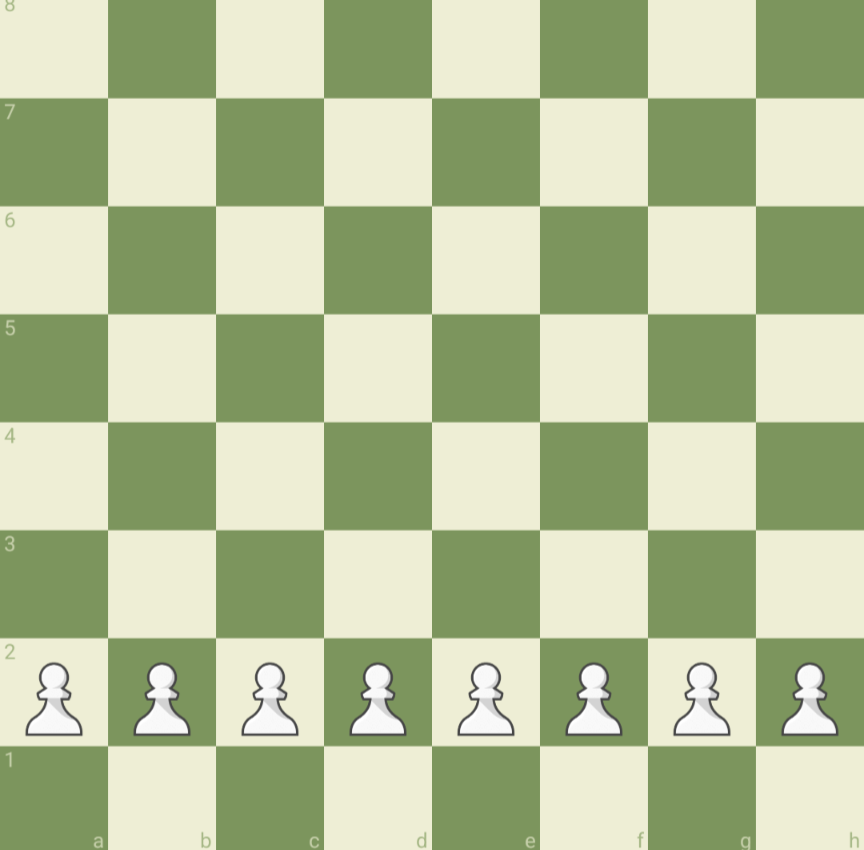
\includegraphics[scale=0.25]{White_Pawns_start.png}
  \centering
  \caption{Starting position for white pawns}
  \label{whitepawns}
\end{figure}

Immediately we may notice that a chess board has dimensions
$(8 \, \textrm{x} \, 8)$ and 64 squares. Furthermore, 
each of the squares in figure \ref{whitepawns} exists 
in one of these two states: There either is a white pawn on
this square or there is not. Does this remind you of a 
familiar concept in computer science? This innate similarity to 
the binary numbering system motivates one to consider the 
use of binary in order to represent a chess board. We can take a 
64 bit unsigned integer and have each \texttt{0} 
represent the lack of a piece and similarly 
have each \texttt{1} represent the existance of a piece on 
this square.\\

Consider the following code snippet.\footnote{The importing
of the numpy library has been omitted for clarity.}

\begin{minted}[linenos, bgcolor=lightgray]{Python}
  # For the rest of this paper i64 will refer to the 
  # unsigned 64 bit integer
  i64 = np.uint64
  WhitePawn = i64(0b        # Dots represent 0,
                  00000000  # . . . . . . . .
                  00000000  # . . . . . . . .
                  00000000  # . . . . . . . .
                  00000000  # . . . . . . . .
                  00000000  # . . . . . . . .
                  00000000  # . . . . . . . .
                  11111111  # 1 1 1 1 1 1 1 1
                  00000000) # . . . . . . . .
\end{minted}

Each bit in the \texttt{WhitePawn} variable represents the
state of a square like we saw previously, this allows us to 
store the state of the board with 12, 64 bit numbers 
(6 piece types in chess, and 2 players). Modern computers
typically have register sizes of 64 bits or greater, 
meaning that we may easily and quickly manipulate these 
bitboards in order to generate legal moves for a position.
We will consider how we may leverage bitboards for legal 
move generation in the following subsection. 
\footnote{We assume reverse little endian indexing for 
our boards throughout.}

\subsection*{Legal move generation}
Legal move generation is the first step to writing a strong
chess engine, in this component we wish to 
find a way to feed in a position to a computer program and have it 
output to us all of the possible legal moves available in this position.
The study of move generation algorithms in the chess programming world 
is still very nascant, with one of the newest algorithms
being discovered in 2017 \cite{bm}. The two algorithms I
decided to spend time researching were
\textit{Hyperbola quintessence} and 
\textit{Magic bitboards} because they are the standard 
accepted algorithms for the top chess engines 
\cite{stockfish}. Both these algorithms are used to generate
moves for sliding pieces 
\footnote{That is the queen, bishop and rook.}.\\

\subsection*{Magic bitboards}
Magic bitboards were discovered in 2006 by Lasse Hansen
\cite{lasse}, and was heavily influenced by Gerd Isenberg's
\textit{"Kindergarten"} bitboards. Both techniques use the
same core idea: we will access moves from a pre-initialised
moves array/table instead of calculating the required move
set on the fly. Magic bitboards involves the usage of a 
\textit{perfect} hash function to map all possible board
occupancies to all their corresponding move sets. By 
occupancy I mean some bitboard of all other pieces that
are able to block the movement of our sliding piece. For 
instance consider a rook on the A1 square, if there is 
another piece on the D1 square the rook will not be able to 
move past D1 anymore. After we hash our occupancy bitboard,
we will use it to index into a pre-calculated attack array
that will give us a bitboard of the correct legal moves in 
$O(1)$ time and space complexity. Examples are often the 
best way to explain concepts so let's go through a simple one.
Let's use our rook that was on A1. It's bitboard will look 
like this:

\newpage
\begin{minted}[linenos, bgcolor=lightgray]{Python}
  WhiteRook = i64(0b        # Dots represent 0,
                  00000000  # 8 |. . . . . . . .
                  00000000  # 7 |. . . . . . . .
                  00000000  # 6 |. . . . . . . .
                  00000000  # 5 |. . . . . . . .
                  00000000  # 4 |. . . . . . . .
                  00000000  # 3 |. . . . . . . .
                  00000000  # 2 |. . . . . . . .
                  10000000) # 1 |1 . . . . . . .
                            #    _______________
                            #    A B C D E F G H
\end{minted}

The technique is no doubt fast, we are simply accessing
an array, the concern with this technique is rather it's
memory consumption.

\subsection*{Hyperbola quintessence}
